This chapter presents a conceptual overview of SDR systems. \autoref{fig:sdr_block_diagram} shows a block diagram of a typical SDR system both from transmitter and receiver sides.
\begin{figure}[ht]
  \centering
  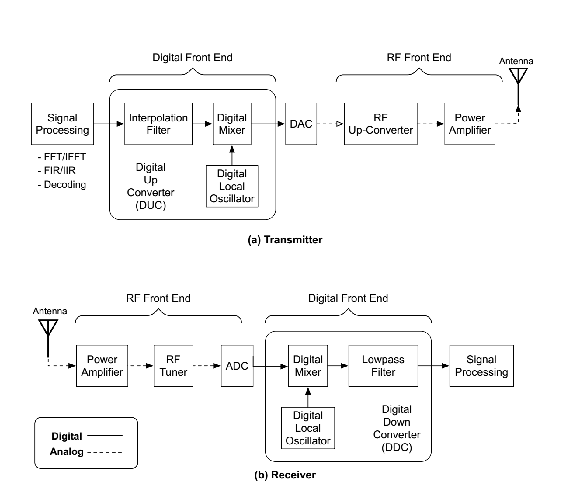
\includegraphics[width=0.75\textwidth]{sdr_block_diagram}
  \caption{Generic SDR architecture [\citeauthor{DBLP:journals/corr/abs-1804-06564}]}
  \label{fig:sdr_block_diagram}
\end{figure}

An SDR transceiver typically consists of the following components: signal processing unit, digital front end, analogue RF front end, and an antenna.
\begin{enumerate}
  \item Antenna: Several types of antennas can be used to cover a wide range of frequency bands \cite{communications_receivers}, depending on the tuning and protocol capabilities of the SDR equipment. A frequent option in LEO satellite reception is the use of rotating antennas to follow the satellite's path. Other technologies that can be very useful in SDR systems are the so called `intelligent' or `smart' antennas that can use mobile tracking (i.e beam-forming capability), and/or interference cancellation (sometimes known as self-healing) \cite{rf_dig_sig_processing} \cite{review_tech_sdr}.

  \item RF front end: This is the RF circuitry responsible for transmitting and receiving the signal at various carrier frequencies. As a minimal structure, it's composed of a local oscillator (LO), a mixing section, and a power section (a power amplifier (PA) in the transmission path and a low-noise amplifier (LNA) in the receiver path). Real-world devices typically include other blocks such as power detectors and filters.
  \begin{enumerate}
    \item In the transmission path the analogue signal is mixed with a local oscillator (LO) signal to produce the RF signal at the preset frequency. It is then amplified using a power amplifier (PA) and transmitted. Advanced techniques such as digital pre-distortion (DPD) or envelope tracking, can be used to maximize output power while maintaining linearity in the PA. Other components that are typically part of this section are impedance matching networks, diplexers and RF filters such as surface acoustic wave (SAW) filters to reduce interference and comply with regulations like, for example, transmission masks.
    \item In the receiver the signal is connected to the RF front end using impedance matching circuitry to avoid signal reflections and ensure maximal power transfer. It is then fed to a low noise amplifier (LNA), which is usually placed close to the antenna, in order to amplify the incoming signal and maximize the SNR. This amplified signal is mixed with the LO signal and converted directly to baseband, or to an intermediate frequency (IF) in the case of heterodyne architectures\cite{tech_radio_handbook}. Other components that can also exist are power detectors for gain control, and RF filters to suppress interference in the form of image frequencies.
  \end{enumerate}

  \item Analogue-to-digital (ADC) and digital-to-analogue (DAC) conversion: The DAC is responsible for producing the analogue signal to be transmitted, from the digital samples. On the receiver side, the ADC performs the inverse operation by converting the continuous-time signal to a discrete-time, binary-coded signals. The devices can operate at baseband or IF, depending on the SDR architecture. ADC performance can be described by various parameters \cite{adc_survey} \cite{digital_frontend_sdr} including: signal-to-noise-and-distortion ratio (SINAD), effective number of bits resolution (ENOB), spurious-free dynamic range (SFDR), among others. These parameters are discussed in more detail, in \autoref{sect:radio_performance_and_impairment}.

  \item Digital front end: The digital front end executes some tasks traditionally implemented in the analogue domain. Two of its main functions are\cite{digital_frontend_sdr}:
  \begin{enumerate}
    \item  Sample rate conversion. Frequently, baseband blocks operate at a much lower frequency than the ADC/DAC devices. This requires an upsampling and interpolation operation (increasing the sample rate), or a decimation and downsampling operation (reducing the sample rate). The decimation filter in the receiver is typically matched to the transmitter's interpolation filter, in order to reduce additive noise. This is known as \emph{matched filtering} and is a common technique to design optimum receiving filters \cite{communication_systems_carlson}.
    \item Channelization. This includes up/down conversion in the transmitter and receiver side. For example in digital IF applications, the digital up converter (DUC) translates the baseband signal to IF, using digital mixer and a numerically-controlled oscillator (NCO). The DAC that is connected to the DUC then converts the digital IF samples into an analogue IF signal. In the receiving side the ADC converts the IF signal into digital samples and these are fed into the digital down converter (DDC) which is composed of a digital mixer and a NCO to obtain baseband digital signal from the IF signal.
  \end{enumerate}

  \item Signal processing: This block is responsible for the signal processing operations, such as forward error correction (FEC) encoding/decoding, interleaving/deinterleaving, modulation/demodulation, and scrambling/descrambling. Another crucial block is the fast Fourier transform (FFT) and inverse FFT (IFFT), which can be used in modulation (for example in orthogonal frequency-division multiplexing (OFDM) systems \cite{ofdm_baseband_receiver}) and other algorithms that operate in the frequency domain (for example, frequency offset compensation algorithms). The signal processing block implementation needs to run on top of hardware circuitry that is able to process these signals very efficiently. Depending on the system specifications these hardware platforms can include general purpose processors (GPPs), graphics processing units (GPUs), digital signal processors (DSPs), field programmable gate arrays (FPGAs) and application-specific integrated circuits (ASICs). Often the most computing-intensive operations can be deployed in dedicated hardware such as an FPGA core. In \autoref{sect:dsp_realizations} a more detailed discussion is presented on the aforementioned hardware platforms and the various design approaches.
\end{enumerate}

The next sections will be dedicated to describing each of the aforementioned SDR sections in more detail (with the exception of the antenna). Prior to that, in \autoref{sect:radio_performance_and_impairment}, a description is made of some general concepts related to radio performance and impairments, which are important to understand both the characteristics of each SDR architecture, and the results from the applications developed in \autoref{chap:demo_apps}. This section also discusses important parameters related to the ADC/DAC devices. \autoref{sect:sdr_system_architecture} then describes some of the possibilities for SDR topologies in terms of the RF front end and digital front end sections, listing their advantages and disadvantages. These topologies are broadly grouped into three groups:
\begin{enumerate}
  \item RF sampling: architectures which sample the RF signal directly, without first converting to an intermediate frequency or to baseband.
  \item IF sampling: architectures which first convert the signal to an intermediate frequency (usually in the tens of megahertz) and then perform sampling.
  \item Baseband sampling: Architectures which convert the signal to baseband (also known as 0 Hz or DC), and then perform sampling.
\end{enumerate}


Finally, \autoref{sect:dsp_realizations} discusses some of the most common options employed for realization of the signal processing stage (the core of the SDR), describing the advantages and disadvantages of each one.

%%%%%%%%%%%%%%%%%%%%%%%%%%%%%%%%%%%%%%%%%%%%%%%%%%%%%%%%%%%%%%%%%%%%%%%%%%%%%%%
\section{Radio Performance and Impairments}
\label{sect:radio_performance_and_impairment}

This sections describes some RF performance concepts and parameters, which are important when understanding the different SDR architectures, and when evaluating the performance of the developed algorithms and applications.

One of the most important parameters is the \emph{signal-to-noise ratio} (SNR) which defined as the ratio of the total signal power to the total noise power:
\begin{align}
  \text{SNR} = \frac{S}{N} = \left(\frac{S_{rms}}{N_{rms}}\right)^2
\end{align}
where
\begin{itemize}
  \item $S$ = Input signal power, in Watt
  \item $N$ = Noise power, in Watt
  \item $S_{rms}$ = Root-mean-square (RMS) amplitude of input signal
  \item $N_{rms}$ = RMS amplitude of noise
\end{itemize}

\noindent Power, noise and SNR are often expressed in logarithmic units, rather than linear units:
\begin{align}
  \text{SNR(dB)} = 10\log(SNR) =  10\log(S) - 10\log(N) = S\text{(dBm)} - N\text{(dBm)}
\end{align}

When analysing SDR systems, two of the most important components are ADC and the DAC. To analyse these, a common set of parameters is typically employed by manufacturers, which facilitates comparison between devices (although sometimes insufficient testing conditions information, such as signal frequency range, bandwidth and repetition, makes it difficult to obtain a trustworthy comparison). One of these parameters is the \emph{total harmonic distortion} (THD), which is defined as the ratio of the RMS value of the fundamental signal to the equivalent RMS of its harmonics (generally, only the first 5 harmonics are significant). THD of an ADC is usually measured in dBc and generally specified with the input signal close to full-scale, although it can be specified at any level.
\begin{align}
  \text{THD} = \frac{S_{rms}}{D_{rms}} = \frac{S_{rms}}{\sqrt{H_{1_{rms}}^2+H_{2_{rms}}^2+H_{3_{rms}}^2+H_{4_{rms}}^2+H_{5_{rms}}^2}}
\end{align}
where $D_{rms}$ represents distortion introduced by the harmonics.

\emph{Spurious free dynamic range} (SFDR) is another parameter, defined as the ratio of the RMS value of the input signal to the RMS value of the worst spurious signal regardless of where it falls in the frequency spectrum. The worst spur may or may not be a harmonic of the original signal. SFDR is an important specification in communications systems because it represents the smallest value of signal that can be distinguished from a large interferer. SFDR can be specified with respect to full-scale (dBFS) or with respect to the actual signal amplitude (dBc). \autoref{fig:sfdr_plot} illustrates how SFDR can be measured.

\begin{figure}[ht]
  \centering
  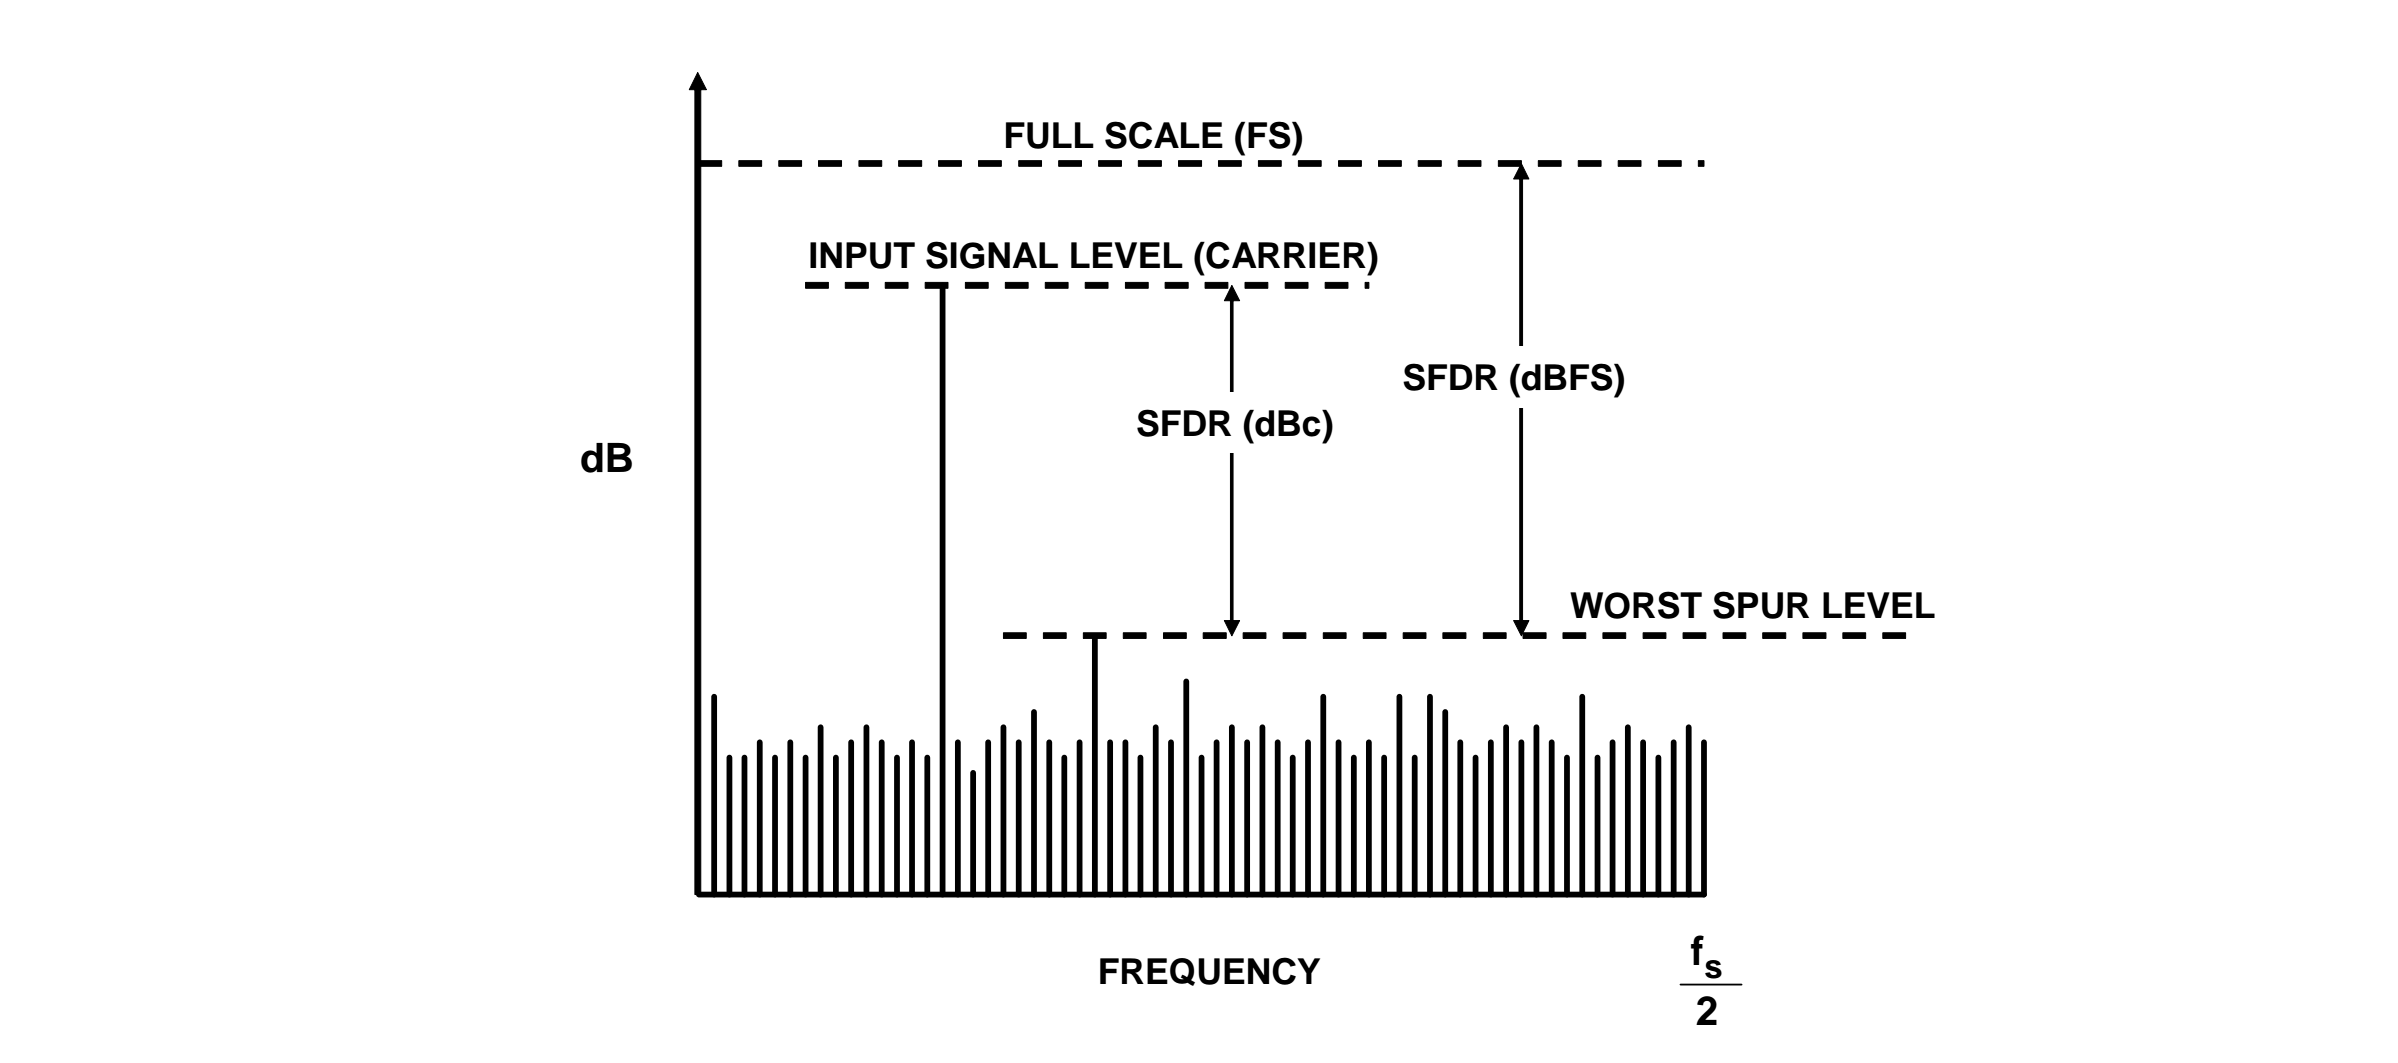
\includegraphics[width=\textwidth]{sfdr_plot}
  \caption{Spurious Free Dynamic Range [\citeauthor{understand_sinad}]}
  \label{fig:sfdr_plot}
\end{figure}

Finally the \emph{signal to noise and distortion ratio} (SINAD) is defined as the ratio of the RMS value of the input signal to the RMS value of all other spectral components including harmonics (but excluding DC):
\begin{align}
  \text{SINAD} = \frac{S_{rms}}{D_{rms}+N_{rms}}
\end{align}

SINAD is a good indicator of the dynamic performance of ADCs since it includes all components that make up noise and distortion. This parameter can also be related to the number of bits of the ADC using the theoretical ideal model of an ADC which assumes that only quantization noise exists and that it approximates AWGN \cite{improve_adc_res}:
\begin{align} \label{eq:SNR_ADC_dB}
  \text{SINAD(dB)} = (6.02 \cdot N_b) + 1.76
\end{align}
where $N_b$ is the number of bits of the ADC. It's important to note that \eqref{eq:SNR_ADC_dB} assumes a full-scale input signal as well. Finally, oversampling and averaging can be employed to reduce the in-band noise and hence increase the SINAD. In this case $N_b$ in \eqref{eq:SNR_ADC_dB} is replaced by the \emph{effective number of bits} (ENOB). Without going into the full detail, one can state a simple, but useful, rule of thumb:

\begin{displayquote}
  \emph{Each doubling of the sampling frequency will lower the in-band noise by 3 dB, and increase the resolution of the measurement by $1/2$ bit.}
\end{displayquote}

Note that whenever one is looking at a signal in the frequency domain, that's been obtained through an FFT, it's important to take into account the effects of the window used, namely the apparent attenuation caused by the signal not being contained within a single FFT bin (an effect known as \emph{scalloping loss}). Full analysis in beyond the scope of this thesis but can be consulted in \cite{harris_windows}.

SNR (or SINAD) can also be related to digital domain parameters. Closely related to the SNR is the $E_s$/$N_0$ parameter which is the ratio between the symbol energy and the noise spectral density. This parameter can be defined (in dB), and related to the SNR, as follows:
\begin{align}
  \frac{E_s}{N_0} (\text{dB}) & = 10\log_{10}\left(S\frac{T_{s}}{(N/B_n)}\right) \nonumber \\
                              & = 10\log_{10}\left(T_{s}F\left(\frac{S}{N}\right)\right) \nonumber \\
                              & = 10\log_{10}\left(\frac{T_{s}}{T}\right) + \text{SNR(dB)}
\end{align}
where
\begin{itemize}
  \item $T$ = Sampling period, in seconds
  \item $T_s$ = Symbol period, in seconds
  \item $S$ = Input signal power, in Watt
  \item $N$ = Noise power, in Watt
  \item $B_n$ = Noise bandwidth, in Hz $= F = 1/T$.
  \item $F$ = Sampling frequency, in Hz
\end{itemize}

$E_s/N_0$ can also be expressed in terms of the closely related ratio of the bit energy to the noise spectral density $E_b/N_0$ as
\begin{align}
  \label{eq:esn0}
  E_s/N_0 = E_b/N_0 + 10\log_{10}(k)
\end{align}
where $k$ is the number of information bits per symbol. Note that $k$ depends on the size of the modulation and the code rate of an error-control code. As an example, using a $4/7$-rate code and 16-QAM modulation, $k$ is $\log_2(16) (4/7) = 16/7$, the product of the number of bits per symbol and the code rate.

Finally, and perhaps most important, is the notion of channel capacity famously introduced by Shannon \cite{shannon_capacity}. The information capacity of a channel of bandwidth $B$ (in Hz) with AWGN noise of power spectral density $N_0/2$ is given by
\begin{align}
  C = B\log_{2}\left(1+\frac{P}{N_0 B}\right)
\end{align}
where $P$ is the average transmitted power.

Note that the dependency on bandwidth $B$ is \emph{linear} but the dependency on SNR, $\frac{P}{N_0 B}$, is \emph{logarithmic}. This leads to an insightful conclusion:

\begin{displayquote}
  \emph{To increase the capacity of a communications systems it's easier to expand the bandwidth of the channel than to increase the transmitted power, for a given noise variance}.
\end{displayquote}

From this results it's possible to derive the familiar plots that relate SNR (or $E_b/N_0$) to bit-error rate (BER) which provide a very useful visual representation of the performance of digital modulations. \autoref{fig:PSK_BER_curves} shows a typical $E_b/N_0$ to BER curve for PSK modulations.

\begin{figure}[ht]
  \centering
  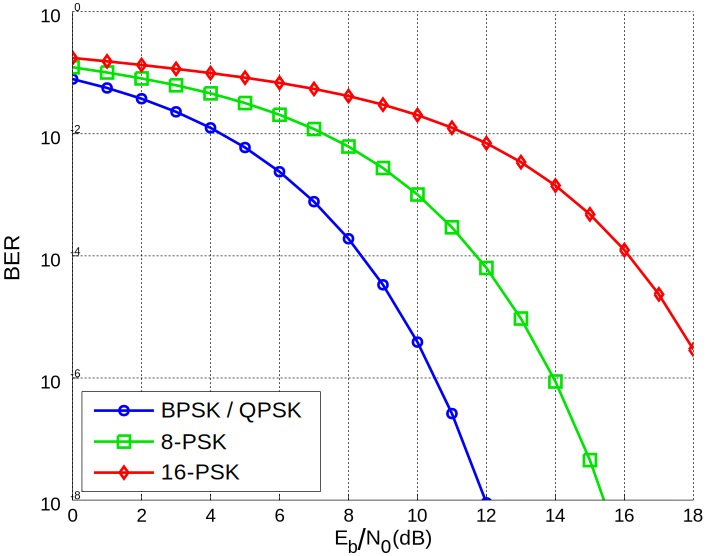
\includegraphics[width=0.75\textwidth]{PSK_BER_curves}
  \caption{Bit-error rate curves for BPSK, QPSK, 8-PSK and 16-PSK, AWGN channel [\citeauthor{image:ber_curve}]}
  \label{fig:PSK_BER_curves}
\end{figure}

Other parameters which are important in RF performance analysis, and are widely used for example in characterising PAs, are the 1-dB compression point (P1dB) and the third-order intercept point (IP3).

An amplifier usually provides a constant gain over a specific frequency range, giving a linear relation between input power and output power. For example, if the gain of an amplifier is 10 dB, then a 1 dBm input signal will result in an 11 dBm output signal. As the input power level increases, there comes a point where the output power of the amplifier no longer increases by the gain value (i.e., the amplifier output power starts to saturate). The P1dB is the output power level at which the gain decreases 1 dB from its constant value \cite{p1db}. Once an amplifier reaches its P1dB it goes into compression and becomes a non-linear device, producing distortion. P1dB is one of the most important specifications for power amplifiers. \autoref{fig:p1db} shows an illustration of the P1dB.

\begin{figure}[ht]
  \centering
  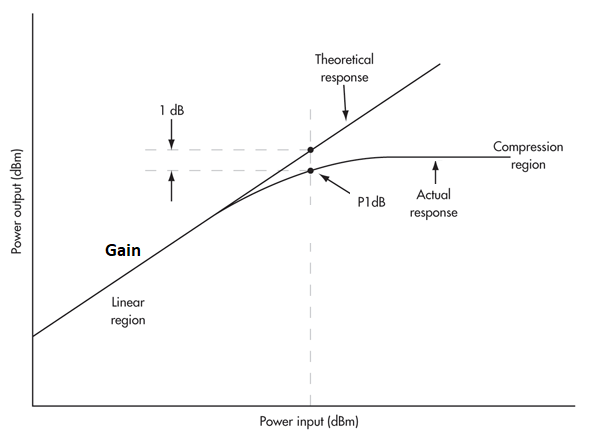
\includegraphics[width=0.6\textwidth]{p1db}
  \caption{1-dB compression point [\citeauthor{p1db}]}
  \label{fig:p1db}
\end{figure}

IP3 is a figure of merit based on the idea that the device nonlinearity can be modelled using a low-order polynomial, derived by means of Taylor series expansion around a small deviation\cite{iip3}. The third-order intercept point relates nonlinear products caused by the third-order nonlinear term to the linearly amplified signal. Its definition can be based on a single tone input or two-tone input.
\begin{itemize}
  \item Based on harmonics: The device is tested using a single input tone. The nonlinear products caused by $n$-th-order nonlinearity appear both at the input tone frequency and at $n$ times it's frequency.
  \item Based on intermodulation products: The device is fed with two sine tones one at $f_1$ and one at $f_2$.  When you cube the sum of these sine waves you will get sine waves at various frequencies including $(2f_2-f_1)$ and $(2f_1-f_2)$.  If $f_1$ and $f_2$ are large but very close together then $(2f_2-f_1)$ and $(2f_1-f_2)$ will be very close to $f_1$ and $f_2$. This two-tone approach has the advantage that it is not restricted to broadband devices and is commonly used for radio receivers.
\end{itemize}
For example, for an input $s_i=S_1 \cos(\omega_1 t)$ and a transfer function given by $s_o=a_1 s_i + a_2 (s_i)^2 + a_3 (s_i)^3$, the cubic term generates
\begin{equation}
  (S_1)^3 (\cos(\omega_1 t))^3 = (S_1)^3 (\frac{3}{4})\cos(\omega_1 t)+\frac{1}{4})\cos(3\omega_1 t))
\end{equation}
The intercept point can then be obtained graphically (\autoref{fig:iip3}) by plotting the output power versus the input power both on logarithmic scales (e.g., decibels). Notice that on a logarithmic scale, the function $x^n$ translates into a straight line with slope of $n$. Therefore, the linearly amplified signal will exhibit a slope of $1$. A third-order nonlinear product will increase by 3 dB in power when the input power is raised by 1 dB. The point where the curves intersect is the intercept point which can be read from the input or output power axis (IIP3 or OIP3).

\begin{figure}[H]
  \centering
  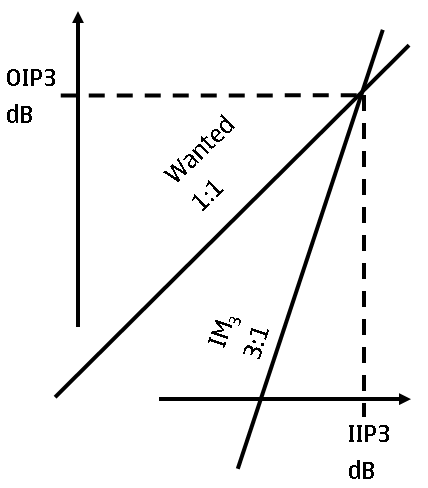
\includegraphics[width=0.4\textwidth]{iip3}
  \caption{Third-order intercept point [\citeauthor{iip3}]}
  \label{fig:iip3}
\end{figure}

Other important parameters, specific to quadrature systems, are \emph{IQ amplitude imbalance} and \emph{IQ phase imbalance}, which have to do with different gain and matching in the I and Q paths of a quadrature system. These will be discussed in more detail in \autoref{sect:sdr_system_architecture}.

%%%%%%%%%%%%%%%%%%%%%%%%%%%%%%%%%%%%%%%%%%%%%%%%%%%%%%%%%%%%%%%%%%%%%%%%%%%%%%%
\section{SDR System Architectures}
\label{sect:sdr_system_architecture}

This section covers some possible architectures in SDR systems, highlighting the main advantages and disadvantages of each one.

\subsection{Ideal SDR System}

The ideal SDR system (shown in \autoref{fig:ideal_sdr}) is one where the entire processing logic is encompassed within the DSP subsystem and the RF section simply needs to amplify and transmit/receive the signal. In this architecture the signal coming from/to the DAC/ADC is already at RF frequency so needs no further up/down conversion. Also, note the ADC and DAC include the anti-alias and reconstruction filters.

\begin{figure}[H]
  \centering
  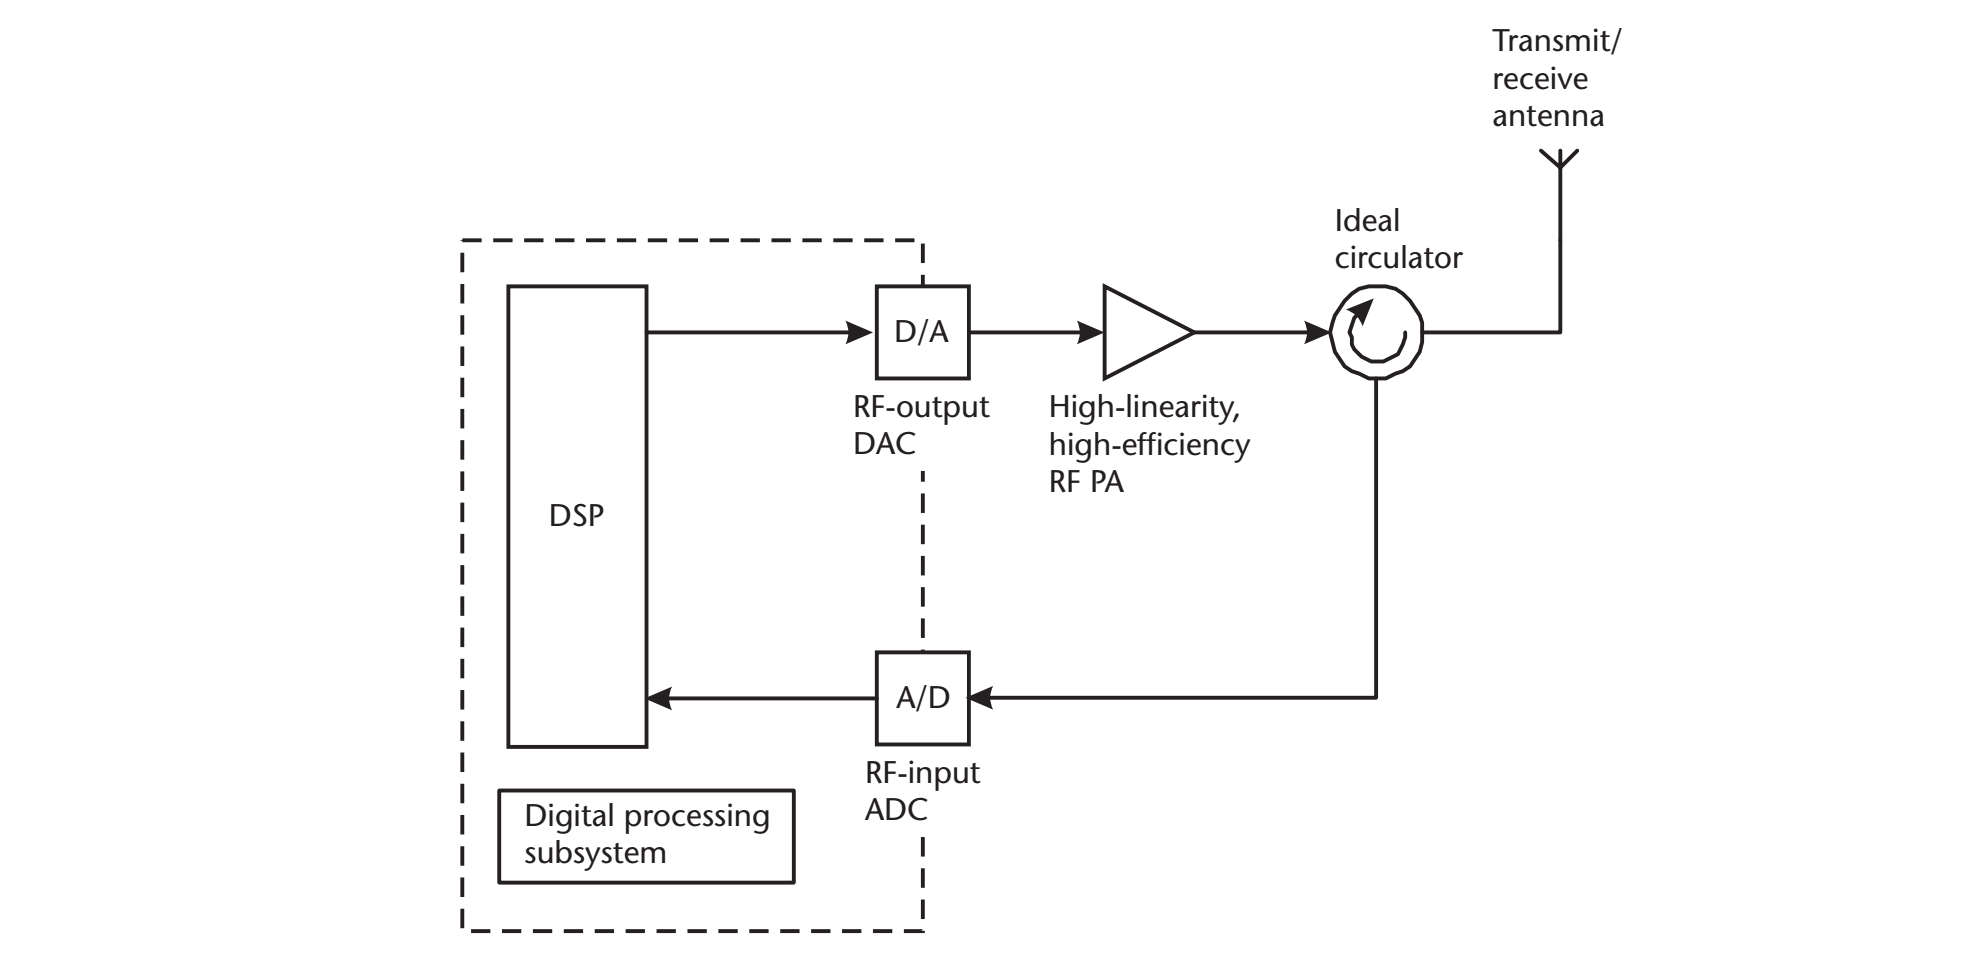
\includegraphics[width=\textwidth]{ideal_sdr}
  \caption[An ideal SDR system]{An ideal SDR system where the entire signal processing (including up/down conversion to the desired RF frequency) is achieved in the DSP subsystem [\citeauthor{rf_bb_techniques_sdr}]}
  \label{fig:ideal_sdr}
\end{figure}

Some of the clear advantages are:
\begin{itemize}
  \item Extremely simplified RF chain.
  \item Elimination of most of the analogue RF related problems such as DC offset, gain/phase imbalance in IQ systems, phase noise from oscillators, among others.
  \item Very high level of flexibility for implementing new protocols and/or when the processing power needs to be upgraded.
\end{itemize}

Unfortunately, technology has not evolved enough to make these systems cost effective. Their chief disadvantage is the fact that they rely on state-of-the-art high-speed ADC/DAC which are very expensive and power demanding (see \autoref{fig:adc12dj2700_power}), compared to a traditional up/down conversion RF chain (even considering the layout engineering effort involved in traditional RF chain design). Note that even if bandpass sampling is employed (which relaxes the sampling frequency requirements of the converters) the large analogue bandwidth necessary at the ADC input (often in the GHz range) is unavoidable if broadband is a requisite. Additionally, the realization of the anti-aliasing filter, which needs to provide sufficient attenuation in the stopband, while being tuned across the entire frequency range, is extremely challenging. As such, this architecture is necessarily reserved for systems where there are no budget restrictions. An RF sampling ADC characteristics page from a well-known vendor is shown in \autoref{fig:adc12dj2700_buy}. In this figure one can observe the very high sampling rate and input bandwidth, among other parameters. Note the full-scale input voltage of the ADC ($V_{FS}$) is just 0.8 V\textsubscript{pp}.

\begin{figure}[H]
  \centering
  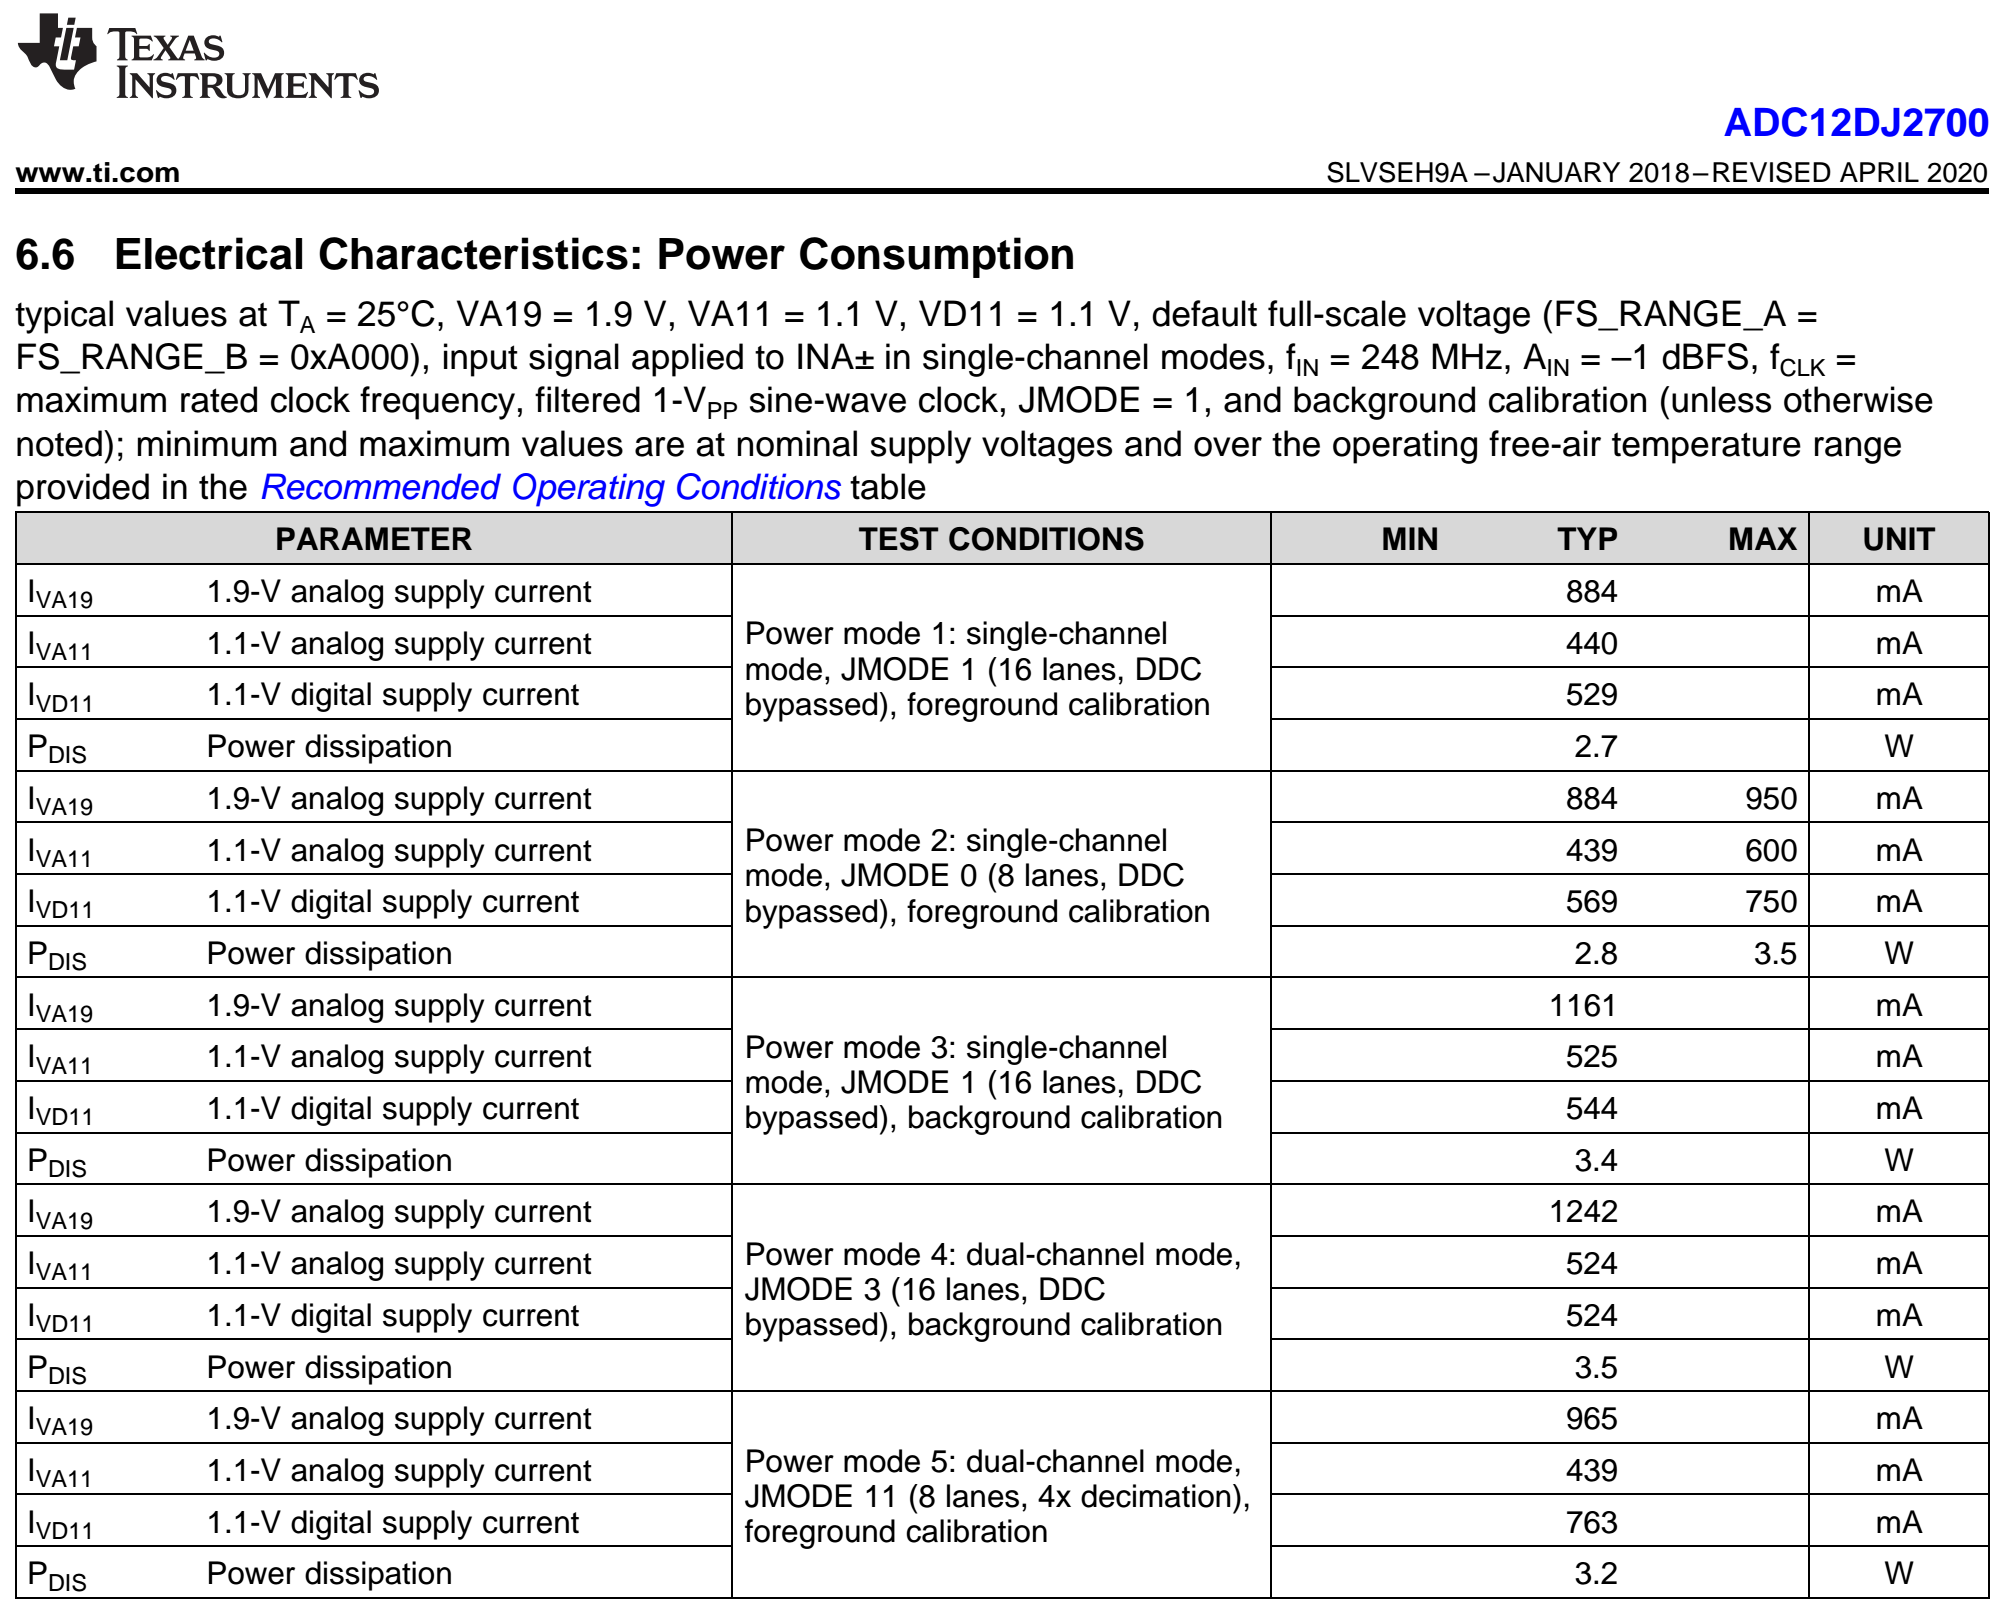
\includegraphics[width=\textwidth]{adc12dj2700_power}
  \caption[TI ADC12DJ2700 power consumption]{An extract from the TI ADC12DJ2700 datasheet, showing the power consumption of the device (from 2.7 W to 3.5 W depending on power mode)}
  \label{fig:adc12dj2700_power}
\end{figure}

\begin{figure}[H]
  \centering
  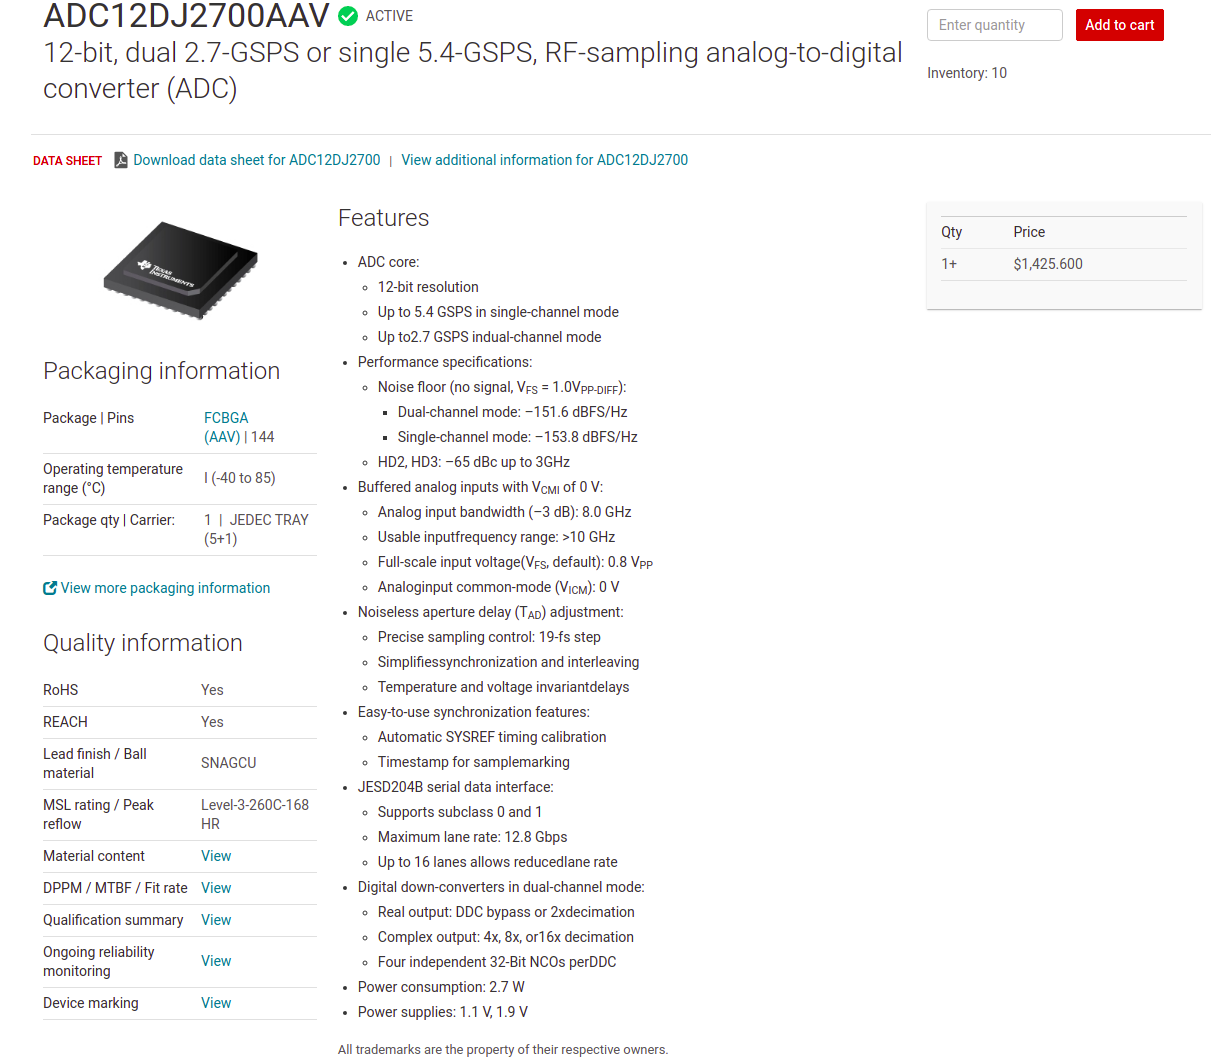
\includegraphics[width=\textwidth]{adc12dj2700_buy}
  \caption[TI ADC12DJ2700 specifications]{The TI ADC12DJ2700, a dual 2.7 GSPS, 12-bit RF sampling ADC which costs \$1425.60 per unit}
  \label{fig:adc12dj2700_buy}
\end{figure}

\subsection{Analogue Quadrature Receiver Architecture}
\label{sect:analogue_quadrature_receiver_architecture}

An alternative approach is seen in \autoref{fig:analog_quadrature_receiver} (only the receive path is shown for simplicity).

\begin{figure}[ht]
  \centering
  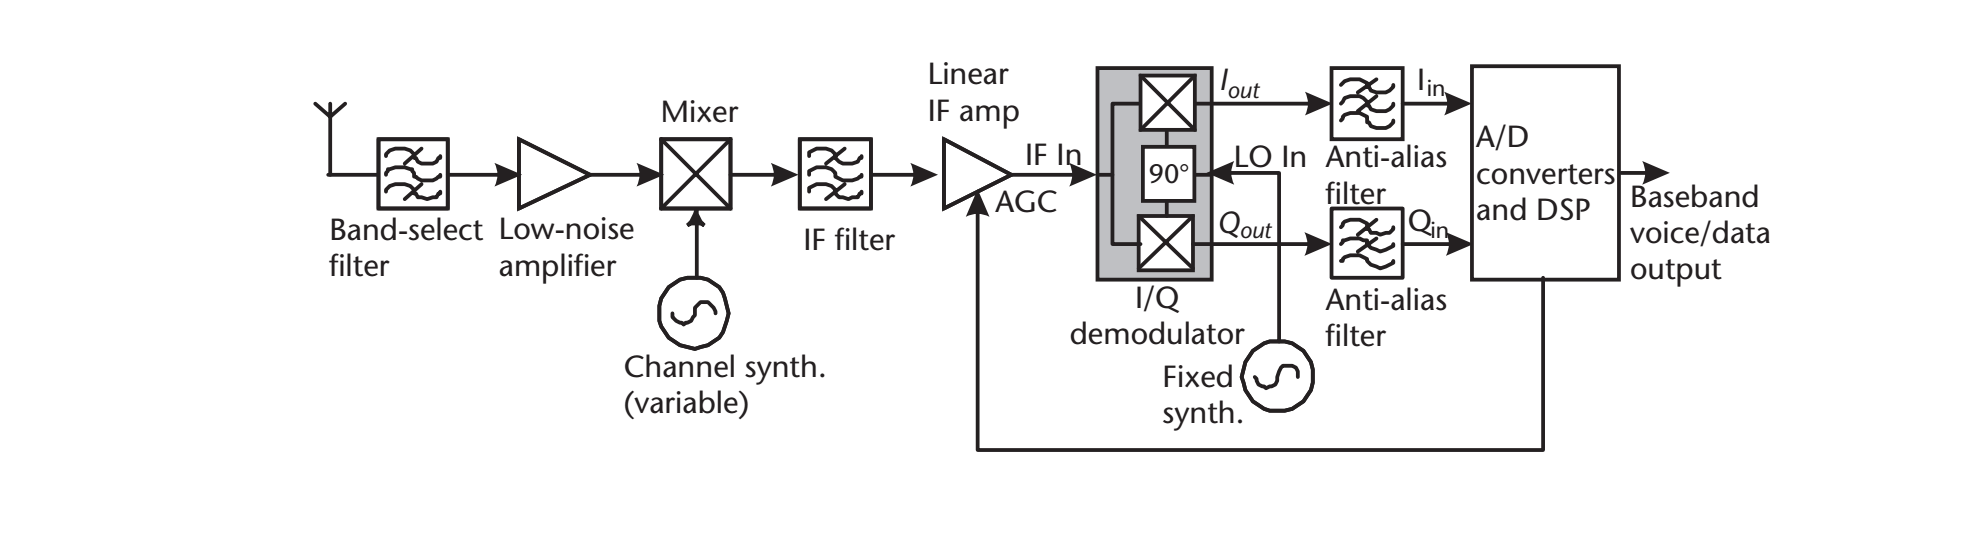
\includegraphics[width=\textwidth]{analog_quadrature_receiver}
  \caption[Analogue quadrature receiver design]{Analogue quadrature receiver design. A common implementation of SDR where the signal modulation and coding is performed in the DSP but the up/down conversion is achieved in the analogue domain [\citeauthor{rf_bb_techniques_sdr}].}
  \label{fig:analog_quadrature_receiver}
\end{figure}

In this case the RF chain needs to amplify and down-convert to IF. After that, the IF filter obtains the desired channel and then the signal is further down-converted to baseband, where the signal is low-pass filtered before being sampled by the ADC. The DSP finally performs the signal demodulation and decoding tasks such as constellation mapping and error correction decoding. The advantages in this architecture are:
\begin{itemize}
  \item Common and well understood architecture. For example, the IF section mitigates the DC offset problem caused by finite isolation between the input and the oscillator mixer ports (common problem in zero IF (ZIF) architecture, see \autoref{sect:zif_arch}).
  \item Transmit/receive path and ADC/DAC with more relaxed requirements can be implemented with relatively low-cost devices. ADC/DAC needs only to accommodate the baseband bandwidth and sampling frequency. Notice that it's becoming more common for the ADC/DAC blocks to include the anti-alias and reconstruction filters in one monolithic package, still maintaining low cost.
  \item Potential for implementing techniques such as oversampling to increase the ENOB and improve SNR.
\end{itemize}

The price to pay is:
\begin{itemize}
  \item Complex analogue path could lead to a slew of problems, especially if care is not taken in the layout phase. Potential for IQ gain and phase imbalance which need to be corrected.
  \item  Multi-stage amplification and filtering leads to the need to a complex mixed signal automatic gain controller (AGC) implementation where the DSP needs to control the analogue section gains in a feedback configuration to avoid saturation (note the figure shows the AGC controlling only the IF amplifier, but more often than not, it needs to control the whole chain, specially the LNA). Multiple oscillators can lead to strict clock requirements and complex architectures for coherent detection.
  \item Changes is system requirements such as different protocols and/or frequency ranges could potentially implicate a full hardware system re-design.
\end{itemize}

\subsection{Digital IF Receiver Architecture}

Perhaps a compromise between the two previous approaches is the \emph{Digital IF } architecture shown in \autoref{fig:digital_if_receiver}. In this realization, the analogue chain ends at the IF stage. The ADC samples directly at IF frequency and the conversion to baseband is performed in software by the DSP, together with the remaining demodulation, error correction and any other signal processing tasks. The IF frequency needs to be sufficiently high to allow channel selection (for example 10 MHz being the minimum requirement, for 3GPP WCDMA, for example), but sufficiently low that it results in achievable A/D and DSP processing bandwidth. This compromise is currently around the 10-50 MHz region, but continues to increase as A/D converter technology evolves.

\begin{figure}[H]
  \centering
  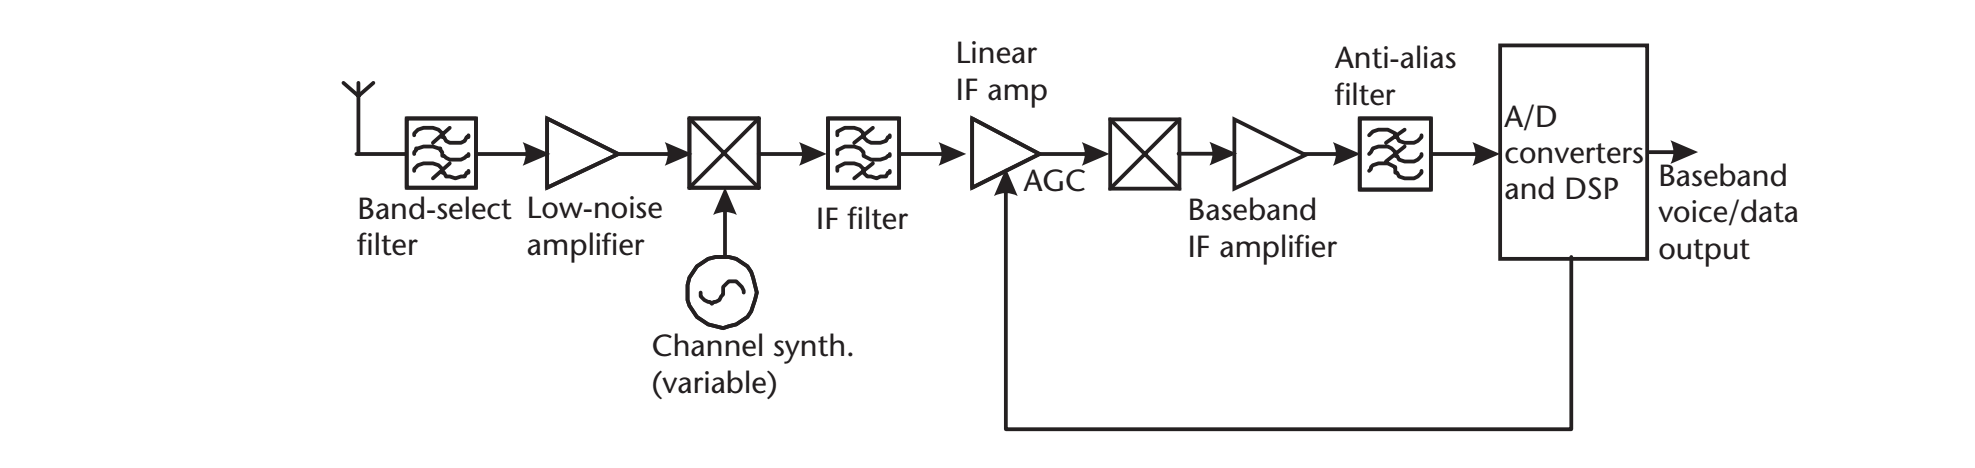
\includegraphics[width=\textwidth]{digital_if_receiver}
  \caption[Digital IF architecture]{Digital IF architecture. The analogue chain ends at the IF section. The ADC sample directly at the IF frequency and the downconvertion is then implemented in the DSP [\citeauthor{rf_bb_techniques_sdr}].}
  \label{fig:digital_if_receiver}
\end{figure}

There are some interesting advantages to this architecture:
\begin{itemize}
  \item Analogue section is confined to a single downconversion stage. The quadrature downconversion can be implemented in the DSP simply by mixing with quadrature numerically-controlled oscillator (NCO) running at $f_s/4$. This can be achieved by multiplying the digital IF samples by the periodic sequences [1, 0, -1, 0] for the in-phase channel and [0, -1, 0, -1] for the quadrature channel, therefore eliminating the problems mentioned in the analogue quadrature receiver architecture. This technique is shown in \autoref{fig:digital_quadrature_demod}.
  \item Simpler considerations for clocks and less analogue blocks to calibrate and control, lead to less requirements and complexity in the firmware.
  \item Potential for power consumption benefits  by having fewer analogue blocks and a simplified power saving logic.
\end{itemize}

The main disadvantages are:
\begin{itemize}
  \item Increased bandwidth necessary at the ADC to sample at IF, therefore possibly limiting other techniques such as oversampling.
  \item High-Q RF filtering section (typically a SAW filter) that needs to reject the image frequency at $f_c \pm f_i$.
\end{itemize}

\begin{figure}[ht]
  \centering
  
\includegraphics[width=\textwidth]{digital_quadrature_demod}
  \caption{Conceptual process of a digital quadrature demodulator [\citeauthor{rf_bb_techniques_sdr}]}
  \label{fig:digital_quadrature_demod}
\end{figure}

\subsection{Zero IF (ZIF) Receiver Architecture}
\label{sect:zif_arch}

In this architecture (also known as a \emph{homodyne receiver}), proposed by Colebrook in 1924 \cite{homodyne}, there is no IF stage, so the signal is directly converted to/from baseband. An example of this technique is shown in \autoref{fig:zif_receiver}.

\begin{figure}[H]
  \centering
  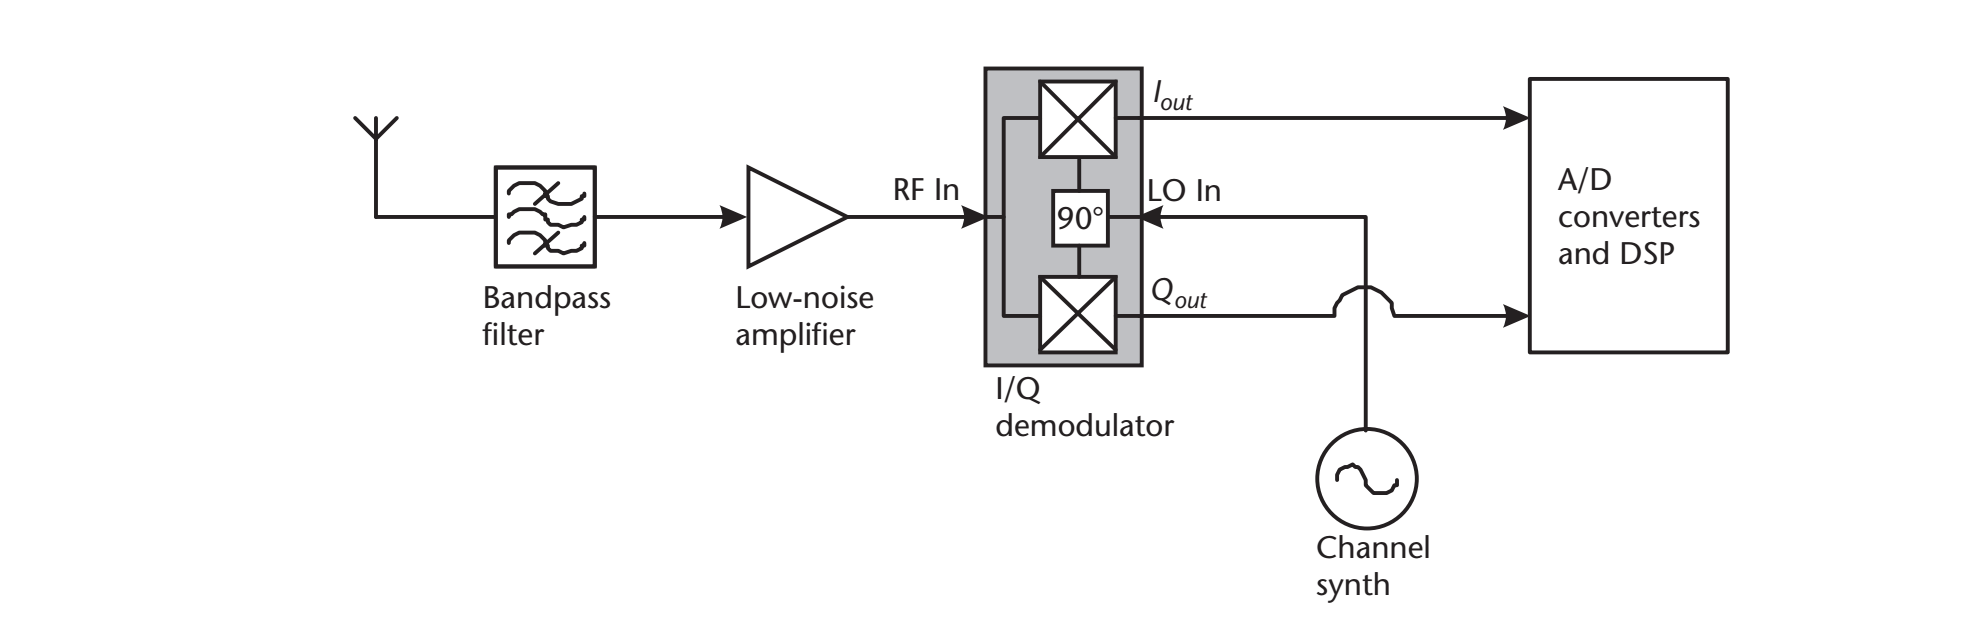
\includegraphics[width=\textwidth]{zif_receiver}
  \caption{Direct Conversion also known as Zero IF Architecture [\citeauthor{rf_bb_techniques_sdr}]}
  \label{fig:zif_receiver}
\end{figure}

This is potentially a very attractive option for the following reasons:
\begin{itemize}
  \item The use of digital filters allows for the implementation of better channel selection filters than could be implemented with analogue IF. In particular, linear-phase filtering is possible, an important property for digital modulation schemes.
  \item The image frequency is in-band and hence the required image-rejection is considerably reduced.
  \item Only a single local oscillator is required, which is advantageous compared to heterodyne systems.
  \item No IF filter is required, hence saving cost and PCB footprint.
\end{itemize}

It does, however, have a number of fundamental problems:
\begin{itemize}
  \item A well designed broadband quadrature network is required, to avoid IQ gain and phase imbalance.
  \item A DC offset appears at the centre of the baseband channel in I and Q and is usually quite high in level with respect to the weaker signals which the receiver may be required to demodulate. This is a consequence of the LO signal leaking to the input port of the mixer and mixing with itself thus appearing at DC. It is caused by finite isolation between LO and input ports in the mixer.
  \item The use of a baseband IF results in problems with low-frequency noise appearing at the centre of the channel ($1/f$ noise).
\end{itemize}

%%%%%%%%%%%%%%%%%%%%%%%%%%%%%%%%%%%%%%%%%%%%%%%%%%%%%%%%%%%%%%%%%%%%%%%%%%%%%%%
\section{Signal Processing Realizations}
\label{sect:dsp_realizations}

SDR signal processing sections are implemented through employing various types of hardware platforms, such as GPPs, GPUs, DSPs, and FPGAs. Each of these has their unique list of challenges. Some of these challenges are:
\begin{itemize}
  \item Making sure there are development tools that allow for an efficient design and implementation process
  \item Efficiently using the the available computational power
  \item Maintaining a low power consumption
  \item Keeping the overall equipment and tools cost low
\end{itemize}

\subsection{GPP}
GPPs are clock-driven and register-based and, for this reason, are capable of different processing functions \cite{microprocessors_and_microcontrollers}. This flexibility makes them tailored to a large number of applications, removing the need for developing application specific circuits. GPPs also allow access to high-level programming languages and well-known frameworks and software packages, making them popular within the scientific community. From the performance point of view, GPPs are being enhanced, due to technological advances in semiconductor technology \cite{lin2014a}, and also to parallelism techniques  in multi-core GPP \cite{ulversoy2010a}. Despite these advances, GPPs cannot match dedicated application-specific platforms for high-throughput computing with real-time requirements, precisely because of their sequential processing model \cite{kamal2003a}. The fact that the GPP often has to switch between different tasks when coupled with an operating system (OS), compromises its performance and can quickly reach saturation with frames becoming corrupted and being discarded. In addition, some protocols require predictable performance in order to guarantee meeting timing constraints. However, conditional branch instructions in GPPs instruction sets lead to out-of-order execution, which makes this difficult to achieve.

In recent years scientists have began to experiment with coupling GPPs wityh GPUs. The latter are specifically designed to handle graphics-related tasks and as such they efficiently process large blocks of streaming data in parallel. This naturraly leads to a model where the act as co-processors for demanding operations, with the GPP typically acting as the control processor. SDR platforms comprised of both GPPs and GPUs have higher processing power but also lower power efficiency than dedicated architectures such as FPGAs (due mostly to the GPP. E.g., GPP's power efficiency is about 9 GFLOPS/W for single precision, compared to 20 GFLOPS/W for GPU \cite{v2014a}). GPUs employ techniques such as \emph{single program multiple data} (SPMD) that allows multiple instruction streams to execute the same program, and \emph{single instruction multiple data} (SIMD) that allows an operation to be performed on multiple data points simultaneously. This makes them good candidates for applications such as video processing.

\begin{table}[ht]
  \caption{Performance of signal detection algorithm on GPP and GPU \cite{fi2017a}}
  \label{table:gpp_gpu_comparison}
  \centering
  \begin{adjustbox}{width=1\textwidth}
  \begin{tabular}{r|r|r|r}
    \toprule
    \multirow{2}{*}{\textbf{ADC Data Length (ms)}} & \multicolumn{3}{c}{Processing Platform of Signal Detection Algorithm} \\
    \multirow{2}{*}{} & \textbf{GPP Serial Processing (ms)} & \textbf{GPP Parallel Processing (ms)} & \textbf{GPU Parallel Processing (ms)} \\
    \midrule
    1    & 13.487    & 1.254    & 0.278 \\
    10   & 135.852   & 12.842   & 2.846 \\
    100  & 1384.237  & 131.026  & 29.358 \\
    1000 & 13946.218 & 1324.346 & 29.358 \\
    \bottomrule
  \end{tabular}
  \end{adjustbox}
\end{table}

In \autoref{table:gpp_gpu_comparison}, the authors of \cite{fi2017a} confirmed that the signal detection algorithm operating in real-time is faster when using a GPU, coupled with the \emph{cuFFT} \cite{cuda_toolkit} library developed by NVIDIA specifically to target efficient FFT computations. This is, in large, due to the fact that the GPU has several thousand \emph{compute unified device architecture} (CUDA) cores that can perform a single operation at the same time (as opposed to a few cores in the case of multi-core GPPs. One caveat is that data operations between GPU and GPP can have limited bandwidth and hence be a source of performance degradation \cite{li2014a}. Recent techniques have been proposed, to ensure no stalls in the pipeline, and thus enhancing processing parallelism \cite{accelerating_massive_mimo_uplink} \cite{millage2010a}.

\subsection{DSP}

A DSP is a particular type of microprocessor that is optimized to process digital signals \cite{rabiner1978a}. Both GPPs and DSPs are capable of implementing complex arithmetic tasks frequently used in communication systems \cite{smith1997a}, such as modulation/demodulation, filtering, and encoding/decoding. DSPs, however, are faster and more efficient due to their architecture which is specifically optimized to handle arithmetic operations, especially additions and multiplications. Examples of DSPs especially designed for SDR platforms are the TI TMS320C6657 and TMS320C6655. Note also that, these DSPs are both equipped with hardware accelerators for specific functionalities which are computationally intensive (such as convolutional and turbo decoders) \cite{unknown-i}, which is a further advantage when compared to GPPs.

\subsection{FPGA}

An FPGA is an array of programmable logic blocks, such as general logic, memory, and multiplier blocks, together with a routing fabric, which is also programmable \cite{kuon2008a}. This type of architecture has the capability of being pre-programmed to implement any design or function and thus acting as an application-specific block. An example of FPGA based SDR platform is the Xilinx Zynq-based implementation of IEEE 802.11ah described in \cite{80211ah_for_iot}, that uses this FPGA board to implement a complete transceiver. Even if FPGAs consume more power and occupy more area than ASICs, the programmability and much lower cost are the main reasons behind their increasing adoption in a wide range of applications. FPGAs are an option that offer the best of both worlds \cite{kuon2008a}, having the performance of ASICs and the programmability of GPPs and DSPs. Despite their lower clock rate (up to about 500 MHz), the fact that FPGAs are designed for specific algorithms and have potential for high level of parallel execution,  increases their performance when compared to GPPs\cite{sano2017a}. A study by \cite{kestur2010a}, confirms that FPGAs out-perform other platform types, such as GPPs and GPUs, in floating point matrix multiplication, both in terms of performance and power efficiency\cite{choi2003a}. For example, the NVIDIA GeForce GTX 980 Ti \cite{unknown-g} is limited to 23 GFLOPS/Watt, compared to the Intel Stratix 10 FPGA which can achieve up to 100 GFLOPS/Watt\cite{altera2010a}.

Traditionally FPGAs are harder to program than GPPs and DSPs due to the employed HDLs such as VHDL and Verilog. These, not only are low-level languages but also require a detailed knowledge of the target hardware architecture. Over the last few years, this has changed as vendors have deployed compilers that can generate FPGA register-transfer level (RTL) code, such as Verilog and VHDL, from high-level programming languages such as C. Some examples include Xilinx HLS \cite{unknown-m} and MATLAB HDL Coder \cite{matlab-a} \cite{unknown-l}.

\subsection{Hybrid}

The hybrid approach, where both hardware and software-based techniques are combined into one platform (also referred to as co-design) has gained a lot of attention in the past few years, since it has become clear that in order to achieve higher performance and realize applications with real-time processing specifications, engineers have to come up with designs that utilize hardware solutions, namely, FPGAs and ASICs \cite{wolf2003a} \cite{micheli2001a} for specific tasks which are computationally intensive, as well as software solutions deployed in GPPs or DSPs. As applications become larger and more complex, more often designers are turning to systems that integrate both software and hardware implementations \cite{teich2012a}. This has been made possible thanks to advances in HLS which can produce efficient RTL from software code, and also define the interface between hardware and software. An example is the Xilinx Zynq platform \cite{unknown-k} which includes two ARM Cortex-A9 processors and also FPGA logic.\cite{unknown-p}.

A high-level comparison between three major design approaches as a guideline is presented in \autoref{table:sdr_approach_comparison}, focusing on the features that are important to SDR design. It shows that, GPPs are easy to program and extremely flexible, they lack processing power to meet real-time specifications and are very power inefficient. Adding multiple cores to the same GPP increases performance by executing more instructions per clock cycle and enabling parallelism. This may not necessarily provide the desired results so an alternative is the addition of GPUs. Sequential algorithms can still execute in multi-core GPP, while computationally intensive portions run on GPU with hundreds or thousands of parallel cores. DSPs out-perform GPPs, and simultaneously maintain ease-of-programmability, making them very interesting options. On the other hand, they are more expensive, which is their chief disadvantage. Finally, FPGAs combine the flexibility of processors with the efficiency of application-specific hardware. FPGAs can achieve high levels of parallelism through reconfiguration, while having superior power efficiency \cite{v2014a}. They are traditionally more suitable for fixed-point arithmetic, like signal processing tasks, but in the recent years their floating-point performance has increased substantially \cite{kestur2010a} \cite{underwood2004a}. The main trade-off is that designers are expected to know a lot more about the hardware.

\begin{table}[ht]
  \caption{Comparison of SDR design approaches [\citeauthor{DBLP:journals/corr/abs-1804-06564}]}
  \label{table:sdr_approach_comparison}
  \centering
  \begin{adjustbox}{width=1\textwidth}
  \begin{tabular}{>{\bfseries}l|c|c|c}
    \toprule
    & \textbf{GPP} & \textbf{DSP} & \textbf{FPGA} \\
    \midrule
    Computation        & Fixed Arithmetic Engines & Fixed Arithmetic Engines & User Configurable Logic\\
    Throughput         & Low                      & Medium                   & High\\
    Execution          & Sequential               & Partially Parallel       & Highly Parallel\\
    Programmability    & Easy                     & Easy                     & Moderate\\
    Complex Algorithms & Easy                     & Easy                     & Moderate\\
    Data Rate          & Low                      & Medium                   & High\\
    Data Width         & Limited by Bus Width     & Limited by Bus Width     & High\\
    I/O                & Dedicated Ports          & Dedicated Ports          & User Configurable Ports\\
    Form Factor        & Large                    & Medium                   & Small\\
    Cost               & Moderate                 & Low                      & Moderate\\
    Power Efficiency   & Low                      & Moderate                 & High\\
    \bottomrule
  \end{tabular}
  \end{adjustbox}
\end{table}
